\documentclass[11pt,a4paper]{article}

\usepackage[utf8]{inputenc}
\usepackage[T1]{fontenc}
\usepackage[french]{babel}
\usepackage{graphicx}
\usepackage{overpic}
\usepackage{hyperref}
\usepackage{geometry}
\geometry{margin=2.5cm}

\title{Introspection et Débogage avec \texttt{pal\_statistics} dans \texttt{ROS
2 Control}} \author{Maximilien Naveau \& Pierre
Fernbach\thanks{firstname.lastname@pal-robotics.com, PAL FRANCE}}
\date{}

\begin{document}

\maketitle

\section*{Durée}

Présentation standard ($\approx$20 minutes), 10 à 15 minutes de présentation + 5
à 10 minutes de questions/réponses.

\section*{Résumé ($\leq$100 mots)}

Cette présentation expose l'intégration de \texttt{pal\_statistics} au sein de
\texttt{ROS 2 Control} pour offrir une introspection \textbf{en temps réel} des
entrées et sorties des contrôleurs. Cette fonctionnalité permet aux développeurs
de surveiller les signaux internes \textbf{sans intervention utilisateur},
améliorant considérablement les workflows de débogage et de réglage. Au-delà de
\texttt{ROS 2 Control}, \texttt{pal\_statistics} peut être utilisé
indépendamment pour exposer des métriques que des outils comme
\texttt{PlotJuggler} peuvent analyser facilement. Nous présentons une
démonstration—implémentée dans \texttt{ros2\_control\_demos}—où nous exécutons
\texttt{ros2\_control\_example\_1} et montrons que chaque contrôleur expose ses
entrées/sorties. Un nœud additionnel est lancé pour illustrer la fonctionnalité
indépendante de \texttt{pal\_statistics} et son utilisation avec
\texttt{PlotJuggler}.

\section*{Description détaillée ($\leq$1000 mots)}

Le débogage et l'introspection sont indispensables pour concevoir des systèmes
robotiques fiables fonctionnant en temps réel. Dans ce contexte, il est
essentiel que les outils et méthodes utilisés n'interfèrent pas avec la boucle
de contrôle du robot, dont la fréquence d'exécution peut atteindre plusieurs
kHz, typiquement jusqu'à 2kHz. Cette cadence élevée génère une quantité
considérable de données de log, rendant crucial l'usage d'outils capables de
filtrer et d'analyser efficacement ces informations tout en préservant la
qualité du contrôle. Notons que l'utilisation des topics ROS 2 classiques n'est
pas adaptée à ces fréquences élevées.

De plus, les contrôleurs dans \texttt{ROS 2 Control} exposent généralement
uniquement leurs interfaces de commande et d'état, tandis que les calculs
intermédiaires internes restent souvent inaccessibles aux développeurs. Cette
limitation complique l'identification des goulets d'étranglement, des problèmes
numériques ou des erreurs de configuration lors du développement.

Pour répondre à ces enjeux, PAL Robotics a développé \texttt{pal\_statistics},
une bibliothèque légère conçue pour publier efficacement des métriques et
statistiques arbitraires, même à des fréquences élevées comme 2kHz. Le framework
\texttt{ROS 2 Control} intègre désormais \texttt{pal\_statistics} directement
dans sa couche d'interface contrôleur, permettant à chaque contrôleur d'exposer
instantanément ses entrées, sorties et états internes, sans ajout de code
utilisateur.

Cette intégration apporte plusieurs bénéfices :
\begin{itemize}
  \item \textbf{Introspection automatique :} Chaque contrôleur publie en continu
        ses entrées et sorties par défaut, même à haute fréquence.
  \item \textbf{Transparence des métriques internes :} Les développeurs accèdent
        facilement aux métriques internes, ce qui accélère et clarifie le
        débogage.
  \item \textbf{Outils de visualisation adaptés :} Des outils comme
        \texttt{PlotJuggler} peuvent analyser et afficher ces métriques en temps
        réel grâce aux dernières évolutions ($\leq$3.10.11).
  \item \textbf{Utilisation flexible :} \texttt{pal\_statistics} peut également
        être utilisé indépendamment de \texttt{ROS 2 Control} dans n'importe
        quel n\oe{}ud ROS 2, assurant une introspection cohérente sur l'ensemble des
        sous-systèmes robotiques.
\end{itemize}

\subsection*{Cas d'utilisation exemple}

Pour la démonstration en direct, nous utiliserons
\texttt{ros2\_control\_example\_1} pour exécuter le contrôleur de trajectoire
articulaire sur le rrbot. Avec \texttt{PlotJuggler}, nous montrerons comment les
signaux d'état d'entrée/sortie sont visualisés pour chaque contrôleur en temps
réel. Pour illustrer davantage la flexibilité de \texttt{pal\_statistics}, nous
ajouterons un simple nœud Python qui utilise \texttt{pal\_statistics}
indépendamment de \texttt{ROS 2 Control}, interagissant avec la configuration
example\_1. Cela montrera comment les métriques peuvent être exposées et
visualisées en dehors du framework contrôleur, offrant un workflow
d'introspection cohérent.

Petit example de ce qu'on peut voir une fois les controllers lancés:

Petit exemple de ce que l'on peut voir une fois les contrôleurs lancés :
\begin{figure}[h!]
  \centering
  % Partie gauche : écran vide avec la sélection superposée
  \begin{minipage}[t]{0.49\textwidth}
    \centering
    \begin{overpic}[width=0.95\linewidth]{plot-juggler-empty.png}
      \put(30,5){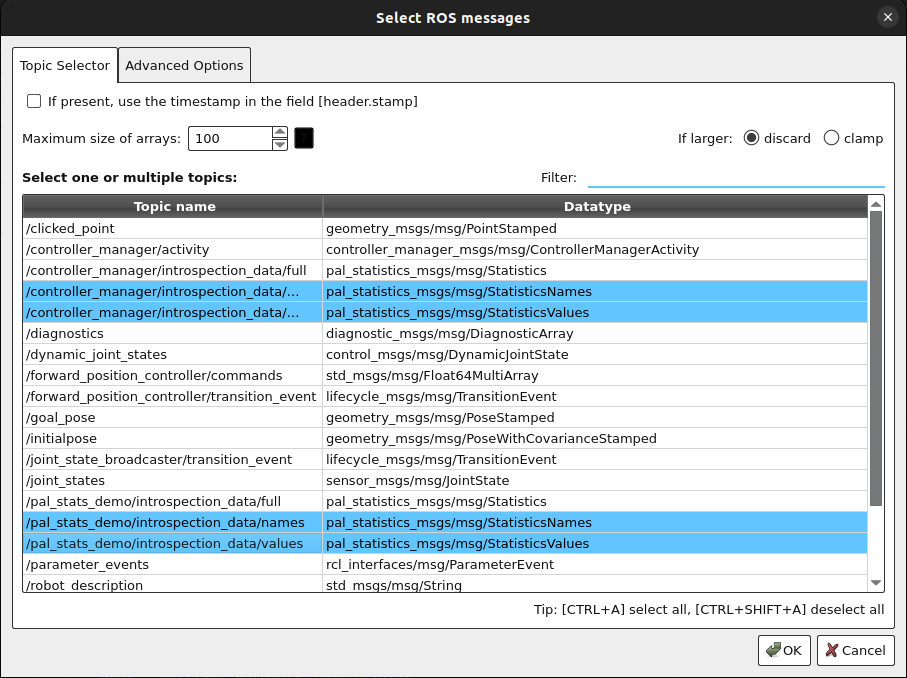
\includegraphics[width=0.6\linewidth]{plot_juggler_selection_with_node.png}}
    \end{overpic}
    \caption*{À gauche : sélection dans PlotJuggler des deux topics d'introspection.}
  \end{minipage}
  % Partie droite : données
  \begin{minipage}[t]{0.49\textwidth}
    \centering
    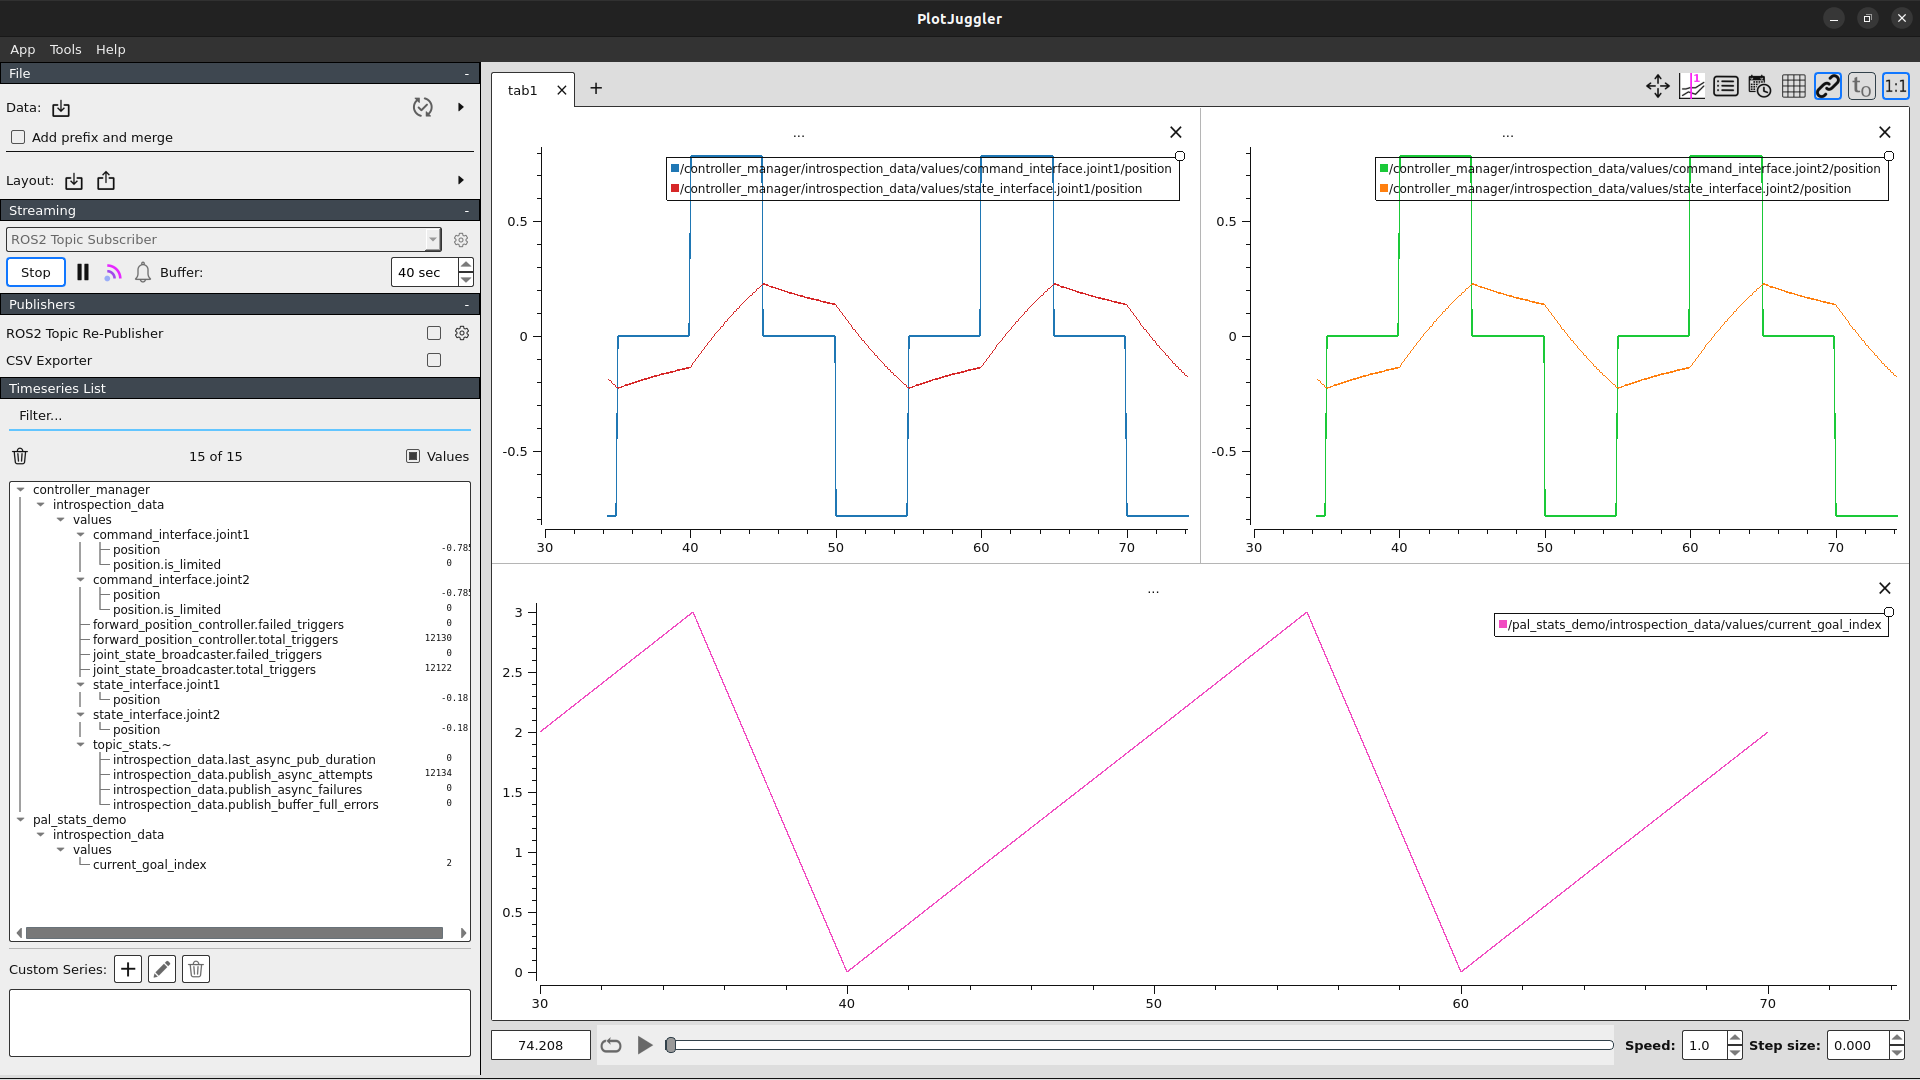
\includegraphics[width=0.95\linewidth]{plot_juggler_2_introspection.png}
    \caption*{À droite : Tracé des signaux d'entrée/sortie des contrôleurs en haut, et tracé du nœud Python en bas.}
  \end{minipage}
  \caption{Exemple d'utilisation de PlotJuggler pour l'introspection en temps réel des contrôleurs ROS 2}
\end{figure}

\subsection*{Points clés pour l'audience}

\begin{itemize}
    \item Comprendre comment \texttt{pal\_statistics} s'intègre dans
          \texttt{ROS 2 Control} pour l'introspection automatique.
    \item Découvrir comment utiliser \texttt{pal\_statistics} indépendamment
    dans des nœuds ROS 2 personnalisés.
    \item Apprendre à visualiser et à déboguer les internes des contrôleurs avec
          \texttt{PlotJuggler}.
\end{itemize}

\section*{Ressources}
\begin{itemize}
    \item \texttt{pal\_statistics} :
    \href{https://github.com/pal-robotics/pal_statistics}{github.com/pal-robotics/pal\_statistics}
    \item \texttt{ROS 2 Control} :
    \href{https://github.com/ros-controls/ros2_control}{github.com/ros-controls/ros2\_control}
    \item \texttt{PlotJuggler} Changelog 3.10.11 :
    \href{https://github.com/facontidavide/PlotJuggler/blob/main/CHANGELOG.rst}{github.com/facontidavide/PlotJuggler/CHANGELOG.rst}
    \item Dépôt de démonstration :
    \href{https://github.com/ros-controls/ros2_control_demos}{github.com/ros-controls/ros2\_control\_demos}
    \item Intégration \texttt{ROS 2 Control} :
    \href{https://github.com/ros-controls/ros2_control/blob/master/hardware_interface/include/hardware_interface/introspection.hpp}{hardware\_interface/include/introspection.hpp}
    \item Intégration \texttt{ROS 2 Control} :
    \href{https://github.com/ros-controls/ros2_control/blob/master/controller_interface/src/controller_interface_base.cpp#L180C3-L180C38}{controller\_interface/controller\_interface\_base.cpp}
    \item Dépôt de la démonstration prévue :
    \href{https://github.com/MaximilienNaveau/roscon-fr-2025}{github.com/MaximilienNaveau/roscon-fr-2025}
\end{itemize}

\end{document}
